%% ------------------------------------------------------------------------- %%
\chapter{Modelo de processo de software}
\label{cap:modeloprocesso}

%% ------------------------------------------------------------------------- %%
\section{Processo de aquisição}
\label{sec:aquisicao}

Segundo a NBR ISO/IEC 12207:1998 \cite{iso12207:95}, o processo de aquisição é composto pelas seguintes atividades:

\begin{enumerate}
  \item Iniciação
  \item Preparação de pedido de proposta
  \item Preparação e atualização do contrato
  \item Monitoração do fornecedor
  \item Aceitação e conclusão
\end{enumerate}

Segundo o item 5.1.1.1 da ISO \cite{iso12207:95}, o adquirente (Gino) inicia o processo com a
descrição de um conceito ou necessidade a adquirir. Principais necessidades do adquirente são:

\begin{itemize}
  \item Padronizar catálogo de receitas
  \item Controle de estoque
  \item Controle de disponibilidade de mesas
\end{itemize}

Segundo o item 5.1.1.4, o adquirente (Gino) pode executar a definição e a análise dos requisitos do software por conta própria ou pode manter acordo com um fornecedor para executar essa tarefa. O adquirente optou por manter um acordo com a empresa de software para que seja feita a definição e análise dos requisitos. Documento de visão será criado para detalhar melhor os requisitos e a estrutura organizacional.



%% ------------------------------------------------------------------------- %%
\section{Processo de fornecimento}
\label{sec:fornecimento}

O fornecedor será responsável por analisar todos os requisitos do sistema de acordo com as necessidades levantadas pelo adquirente (Gino), através de um acordo de contrato. A proposta de tipo de contrato terá escopo variável. Quanto à responsabilidade das organizações, o fornecedor deverá atender as necessidades estabelecidas pelo adquirente para o aceite do software desenvolvido e é de responsabilidade do adquirente prover todas as informações e dados ao fornecedor para a definição do produto final.
O fornecedor será responsável por realizar toda a preparação necessária para elaboração do pedido de proposta do cliente, neste caso, o Gino.

Para a elaboração do pedido de proposta, o fornecedor tem a responsabilidade pelos seguintes itens \cite{iso12207:95}:
\begin{itemize}
  \item Requisitos do sistema
  \item Declaração do escopo
  \item Lista de produtos de software
  \item Termos e condições
  \item Restrições técnicas
\end{itemize}

Após prover os itens acima, eles só serão validados mediante aprovação do cliente.

O contrato será confeccionado mediante direitos de uso, de propriedade, de autoria, de garantia e de licença \cite{iso12207:95}. O adquirente terá prioridade no suporte da aplicação por período pré-estabelecido entre as partes. Também fica pré-definido que qualquer alteração ou aditivo que ocorra no contrato, o fornecedor e o adquirente devem estar em comum acordo. Um documento aprovado por ambas as partes deve ser elaborado suportando estas modificações: análise de impacto quanto a prazos, cronograma e custos \cite{iso12207:95}.

A aceitação será realizada de acordo com o descrito em cada item de requisito levantado, durante as entregas parciais. Uma vez que o fornecedor faz uso de um modelo de desenvolvimento que prevê entregas parciais, o adquirente poderá fazer a validação, verificação e aceitação destas entregas evoluindo até a aceitação final do projeto. A monitoração será realizada de acordo com os status das entregas parciais providas pelo fornecedor. 

Segue a descrição das tarefas e atividades do fornecedor para o processo de fornecimento:


\subsection{Iniciação}

Fornecedor conduzirá uma revisão das necessidades levantadas pelo adquirente para decidir ou propor mudanças para a aceitação do contrato (5.2.1.1 e 5.2.1.2) \cite{iso12207:95}.

\subsection{Preparação de resposta}

O fornecedor será responsável por definir todos os requisitos em resposta ao pedido do \textit{Gino}.

\subsection{Contrato}

Contrato terá escopo variável para atender as necessidades do adquirente de acordo com suas prioridades e trabalhar de acordo com o modelo de desenvolvimento da empresa, SCRUM.

\subsection{Planejamento}

\begin{itemize}
  \item Recursos internos para o desenvolvimento do software utilizando o modelo iterativo - SCRUM (5.2.4.4)
  \item Requisitos e prioridades serão descritos pelo documento de Visão (5.2.4.1)
  \item Estrutura organizacional e cada ciclo será definido pelo SCRUM (5.2.4.2 e 5.2.4.5 a.)
  \item Uso do Kanban e diagrama de Burndown para realizar acompanhamento do progresso (5.2.4.5 n.)
  \item Estes diagramas de \textit{Burndown} poderão ser disponibilizados periodicamente ao adquirente para acompanhamento do progresso
  \item Será provido treinamento ao adquirente para a utilização do produto do software (5.2.4.5 o.)
\end{itemize}

\subsection{Execução e controle}

Monitoramento de progresso feito por Kanban e Burndown (5.2.5.3).

\subsection{Revisão e avaliação}

Fornecedor fará uso de um modelo de entregas parciais. O adquirente irá revisar de acordo com a descrição em cada item de requisito levantando durante as entregas parciais.

\subsection{Entrega e conclusão}

O adquirente poderá fazer a validação e aceitação das entregas parciais evoluindo até a aceitação do projeto final.

%% ------------------------------------------------------------------------- %%
\section{Processo de desenvolvimento}
\label{sec:desenvolvimento}

Devido ao conhecimento e experiência do fornecedor (empresa de desenvolvimento de software), foi definido o modelo iterativo SCRUM com metodologias ágeis para o desenvolvimento do software. 

Segue uma descrição das atividades e tarefas do processo de desenvolvimento:

\subsection{Implementação do processo}

Para o desenvolvimento do software para o adquirente, o modelo de ciclo de vida de software definido é o modelo iterativo SCRUM utilizando metodologias ágeis. Para a correta implementação do processo, os desenvolvedores e gerentes deverão ler o livro do SCRUM.

\begin{figure}[!h]
  \centering
  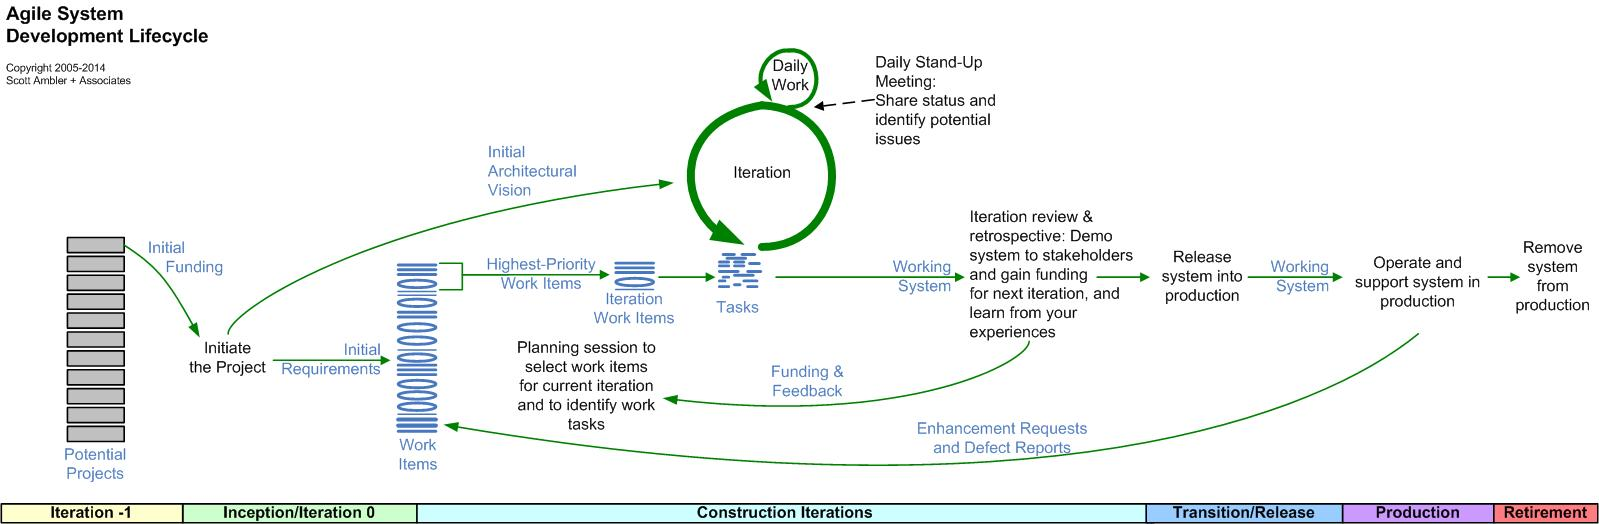
\includegraphics[width=1\textwidth]{lifecyclemodel/images/agileLifecycleDetailed} 
  \caption{Seleção do ciclo de vida ágil baseado no Scrum \cite{ambysoft:09}}
  \label{fig:scrumlifecycle} 
\end{figure}

\subsection{Análise dos requisitos do sistema}

\begin{itemize}
  \item Os requisitos serão definidos pelo fornecedor de acordo com as necessidades levantadas pelo adquirente

  \item Todos os requisitos serão definidos e listados no Product Backlog

  \item Eles serão listados e priorizados pelo PO (Product Owner) e Scrum Master antes do Sprint Planning
\end{itemize}

\subsection{Projeto de arquitetura do sistema}

Mais simples possível, segundo o manifesto ágil \cite{beck2001agile, BecAnd04extreme}. Simplicidade é:
\emph{"A arte de maximizar a quantidade de trabalho não feito."}


\subsection{Análise dos requisitos do software}

O trabalho a ser feito durante o Sprint é definido durante o Sprint Planning juntamente com todo o time de Scrum. No Sprint Planning é definido quais itens serão entregues no próximo Sprint. Estes itens são definidos de acordo com o Product Owner

\subsection{Projeto da arquitetura do sistema}

Manter mais simples possível. A arquitetura deve ser fácil para extender e modificá-la \cite{beck2001agile, BecAnd04extreme}.

\subsection{Projeto detalhado do software}

Mais simples possível para dar liberdade aos desenvolvedores \cite{beck2001agile, BecAnd04extreme}.

\subsection{Codificação e testes do software}

Programação pareada para funcionalidades complexas e TDD (Test driven development).

\subsection{Integração do software}

Integração contínua.

\subsection{Teste de qualificação do software}

Teste de integração ao final de cada sprint.

\subsection{Integração do sistema}

Integração contínua automatizada.

\subsection{Teste de qualificação do sistema}

Teste de acordo com os requisitos do sistema feitas pelo adquirente. Por exemplo, testar o cenário de aviso de pedidos prontos ao garçom num painel.

\subsection{Instalação do software}

Fornecedor irá prover manual de instalação.

\subsection{Apoio à aceitação do software}

O fornecedor irá prover treinamento ao adquirente.


\section{Processo de operação}
\label{sec:operacao}

Segundo a norma NBR ISO/IEC 12207:1998, o processo de operação é composto pelas seguintes atividades:

\begin{enumerate}
  \item Implementação do processo
  \item Teste operacional
  \item Operação do sistema
  \item Suporte ao usuário
\end{enumerate}

\subsection{Implementação do processo}

Para registrar, resolver e rastrear os problemas será utilizado o BugTracking. Problemas identificados serão incluídos no processo de resolução de problemas.%~\ref{sec:resolucao}.

\subsection{Teste operacional}

O teste será feito pelo desenvolvedor juntamente com o adquirente para liberação do produto de software.

\subsection{Operação do sistema}

Será disponibilizado um ambiente com as mesmas condições especificadas pelo adquirente para realizar os testes operacionais.

\subsection{Suporte ao usuário}

As solicitações do usuário, quando necessário, serão encaminhados para resolução no processo de manutenção.

\section{Processo de manutenção}
\label{sec:manutencao}

Segundo a norma NBR ISO/IEC 12207:1998, o processo de manutenção é composto pelas seguintes atividades:

\begin{enumerate}
  \item Implementação do processo
  \item Análise do problema e da modificação
  \item Implementação da modificação
  \item Revisão/aceitação da manutenção
  \item Migração
  \item Descontinuação do software
\end{enumerate}

\subsection{Implementação do processo}
Para registrar, resolver e rastrear os problemas será utilizado o BugTracking. Problemas identificados serão incluídos no processo de resolução de problemas. O gerenciamento do processo de manutenção será feito com Scrum.

\subsection{Análise do problema e da modificação}

O fornecedor fará a análise do problema e da modificação pedida pelo usuário. De acordo com o problema, definirá o nível de criticidade e o prazo para modificar.

\subsection{Implementação da modificação}

Esta atividade será feita pelo desenvolvedor durante a resolução do problema.

\subsection{Revisão/aceitação da manutenção}

O fornecedor fará a revisão junto ao adquirente da modificação solicitada.

\subsection{Migração}

Não haverá migração, pois é um sistema novo.

\subsection{Descontinuação do software}

Caso haja uma descontinuação do software, todos os artefatos gerados durante o ciclo de vida do processo de software serão disponibilizados ao cliente, bem como manuais ou qualquer outro documento que o adquirente tenha requisitado em comum acordo.












